\documentclass{article}
\usepackage{helvet}
\usepackage{geometry}
\usepackage{graphicx}
\usepackage{amsmath}
\usepackage{hyperref}
\usepackage{xcolor}
\usepackage{titlesec}
\usepackage{microtype} % Prevents overfull hboxes by better text wrapping
\geometry{margin=1in}
\usepackage{subcaption}
\usepackage{listings}
\usepackage{color}
\usepackage{float}
% Define colors for code syntax highlighting
\definecolor{codeblue}{rgb}{0.13, 0.13, 0.7}
\definecolor{codegreen}{rgb}{0, 0.5, 0}
\definecolor{codegray}{rgb}{0.5, 0.5, 0.5}
\definecolor{codepurple}{rgb}{0.58, 0, 0.82}

\lstdefinestyle{mystyle}{
    backgroundcolor=\color{white},   
    commentstyle=\color{codegreen},
    keywordstyle=\color{codeblue},
    numberstyle=\tiny\color{codegray},
    stringstyle=\color{codepurple},
    basicstyle=\ttfamily\footnotesize,
    breaklines=true,                 
    captionpos=b,                    
    keepspaces=true,                 
    numbers=left,                    
    numbersep=5pt,                  
    showspaces=false,                
    showstringspaces=false,
    showtabs=false,                  
    tabsize=2
}

\lstset{style=mystyle}

% Define colors
\definecolor{primary}{RGB}{0, 102, 204} % Blue color
\definecolor{IITBBlue}{RGB}{0, 51, 102} % IIT Bombay's signature blue

\usepackage{cite}
\usepackage{amsmath,amssymb,amsfonts}
\usepackage{algorithmic}
\usepackage{graphicx}
\usepackage{textcomp}
\usepackage{xcolor}
\usepackage{hyperref}
\usepackage{placeins}
\usepackage{graphicx}
\usepackage{subcaption}
\usepackage{physics}




\def\BibTeX{{\rm B\kern-.05em{\sc i\kern-.025em b}\kern-.08em
    T\kern-.1667em\lower.7ex\hbox{E}\kern-.125emX}}


\title{Question 4: Assignment 4: CS 663, Fall 2024}
\author{
\IEEEauthorblockN{
    \begin{tabular}{cccc}
        \begin{minipage}[t]{0.23\textwidth}
            \centering
            Amitesh Shekhar\\
            IIT Bombay\\
            22b0014@iitb.ac.in
        \end{minipage} & 
        \begin{minipage}[t]{0.23\textwidth}
            \centering
            Anupam Rawat\\
            IIT Bombay\\
            22b3982@iitb.ac.in
        \end{minipage} & 
        \begin{minipage}[t]{0.23\textwidth}
            \centering
            Toshan Achintya Golla\\
            IIT Bombay\\
            22b2234@iitb.ac.in
        \end{minipage} \\
        \\ 
    \end{tabular}
}
}

\date{October 22, 2024}


\usepackage{amsmath}
\usepackage{amssymb}
\usepackage{hyperref}
\usepackage{ulem,graphicx}
\usepackage[margin=0.5in]{geometry}

\begin{document}
\maketitle

\\

\begin{enumerate}
    \item In this part, you will implement a mini face recognition system. Download the ORL face database from the homework folder. It contains 40 sub-folders, one for each of the 40 subjects/persons. For each person, there are ten images in the appropriate folder named 1.pgm to 10.pgm. The images are of size 92 by 110 each. Each image is in the pgm format. You can view/read the images in this format, either through MATLAB or through image viewers like IrfanView on Windows, or xv/display/gimp on Unix. Though the face images are in different poses, expressions and facial accessories, they are all roughly aligned (the eyes are in roughly similar locations in all images). For the first part of the assignment, you will work with the images of the first 32 people (numbers from 1 to 32). For each person, you will include the first six images in the training set (that is the first 6 images that appear in a directory listing as produced by the \textsf{dir} function of MATLAB) and the remaining four images in the testing set. You should implement the recognition system by using the \textsf{eig} or \textsf{eigs} function of MATLAB on an appropriate data matrix. Record the recognition rate using squared difference between the eigencoefficients while testing on all the images in the test set, for $k \in \{1,2,3,5,10,15,20,30,50,75,100,150,170\}$. Plot the rates in your report in the form of a graph. Now modify the required few lines of the code but using the \textsf{svd} function of MATLAB (on the $\boldsymbol{L}$ matrix as defined in class) instead of \textsf{eig} or \textsf{eigs}. \\
    
    Repeat the same experiment (using just the \textsf{eig} or \textsf{eigs} routine) on the Yale Face database from the homework folder. This database contains about 64 images each of 38 individuals (\textit{labeled from 1 to 39, with number 14 missing; some folders have slightly less than 64 images}). Each image is in pgm format and has size 192 by 168. The images are taken under different lighting conditions but in the same pose. Take the first 40 images of every person for training and test on the remaining 24 images (that is the first 40 images that appear in a directory listing as produced by the \textsf{dir} function of MATLAB). Plot in your report the recognition rates for $k \in \{1,2,3,5,10,15,20,30,50,60, 65,75,100,200,300,500,1000\}$ based on (a) the squared difference between all the eigencoefficients and (b) the squared difference between all \emph{except} the three eigencoefficients corresponding to the eigenvectors with the three largest eigenvalues. Display in your report the reconstruction of any one face image from the ORL database using $k \in \{2,10,20,50,75,100,125, 150,175\}$ values. Plot the 25 eigenvectors (eigenfaces) corresponding to the 25 largest eigenvalues using the subplot or subimage commands in MATLAB. \textsf{[30 points]}

\\
    \makebox[0pt][l]{\hspace{-7pt}\textit{Soln:}} % Aligns "Answer:" to the left
\\
\newpage
All the images are included in the \emph{images} folder, and the code is included in the \emph{code} folder.
\subsection{ORL Face Dataset:}
    \begin{itemize}
        \item using \textbf{eig} function of MATLAB:\\
        \begin{figure}[H]
            \centering
            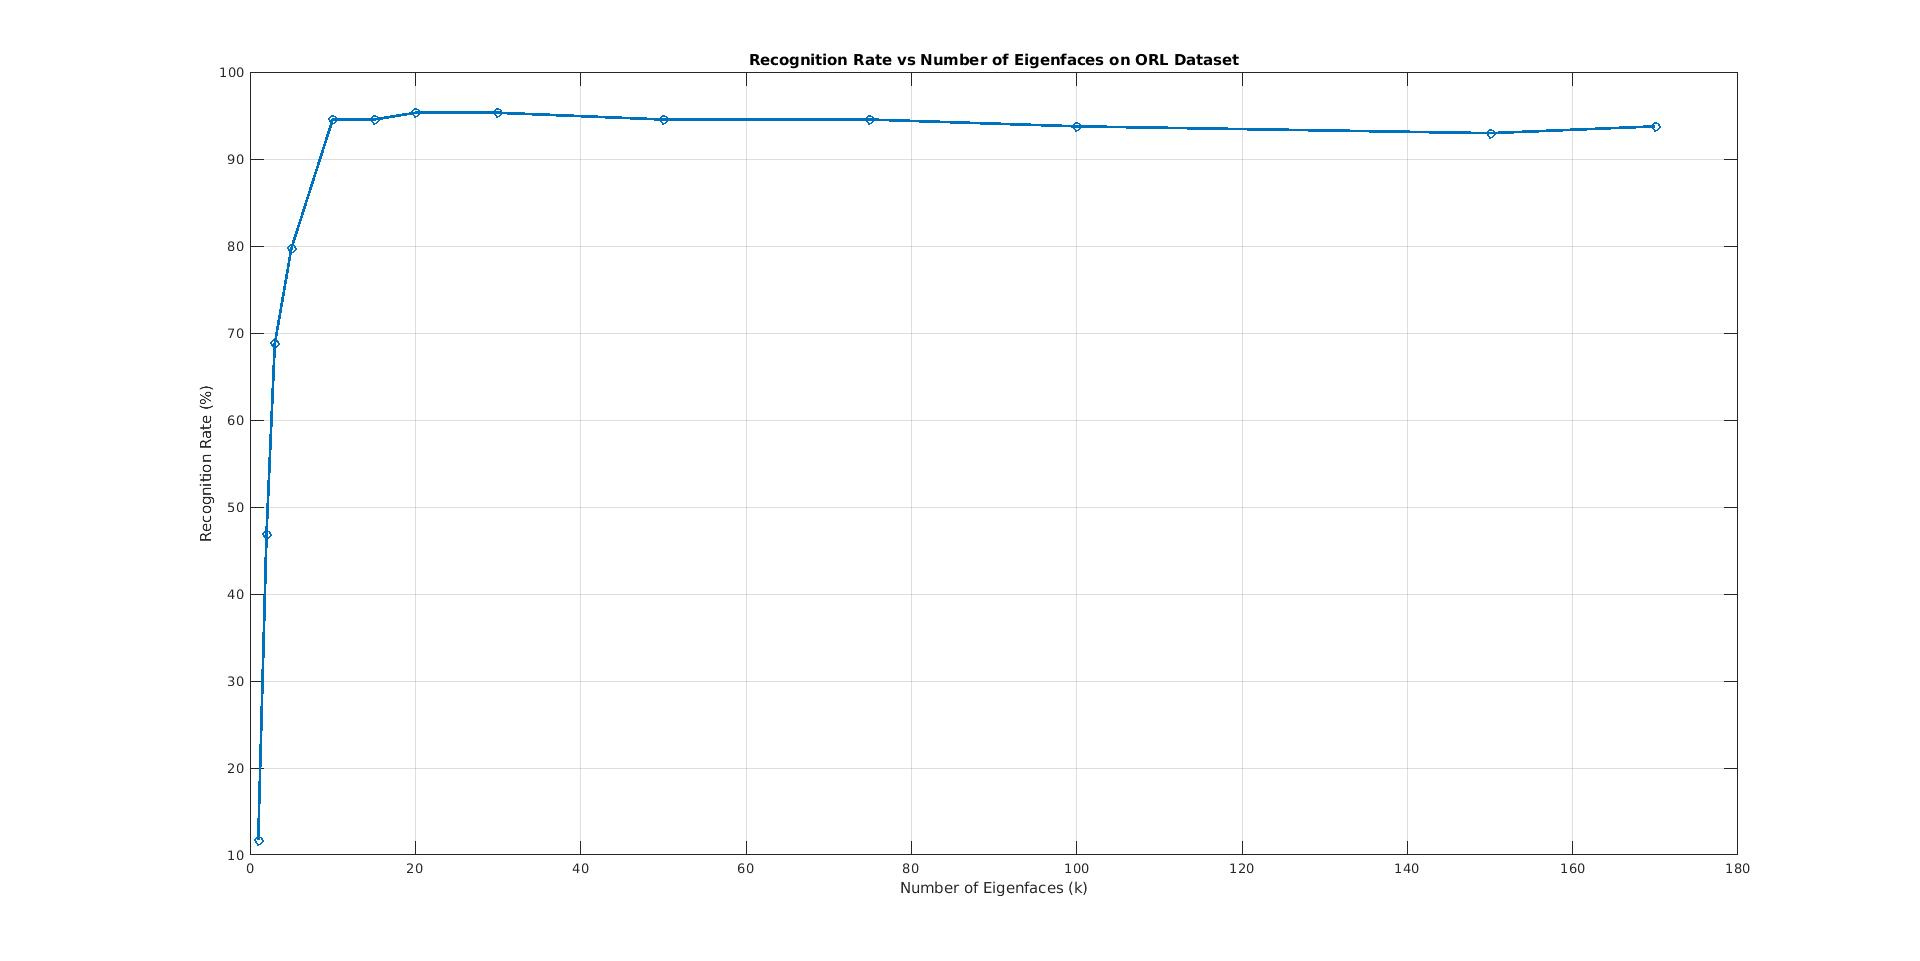
\includegraphics[width=0.9\textwidth]{../images/ORL_dataset_Recognition_Rate_vs_Number_of_EigenFaces.jpg}
            \caption{Recognition rate vs. k using EIG function}
        \end{figure}
        \item using \textbf{svd} function of MATLAB:
        \begin{figure}[H]
            \centering
            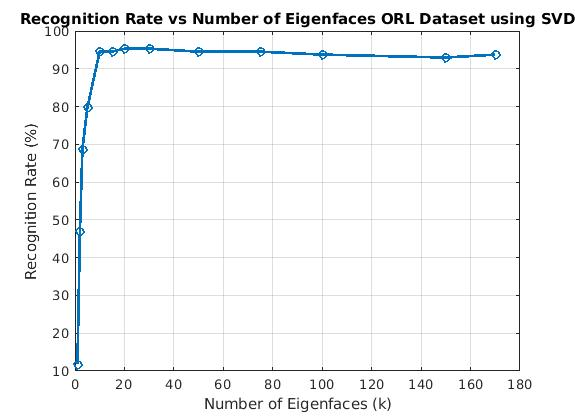
\includegraphics[width=0.8\textwidth]{../images/ORL_dataset_Recognition_Rate_vs_Number_of_EigenFaces_SVD.jpg}
            \caption{Recognition rate vs. k using SVD function}
        \end{figure}
    \end{itemize}
Both the plots are similar. We get maximum recognition rate of 95.3125 for k = 20

\subsection{Yale Face Dataset:}
\begin{itemize}
        \item using \textbf{eig} function of MATLAB:\\
        \begin{figure}[H]
            \centering
            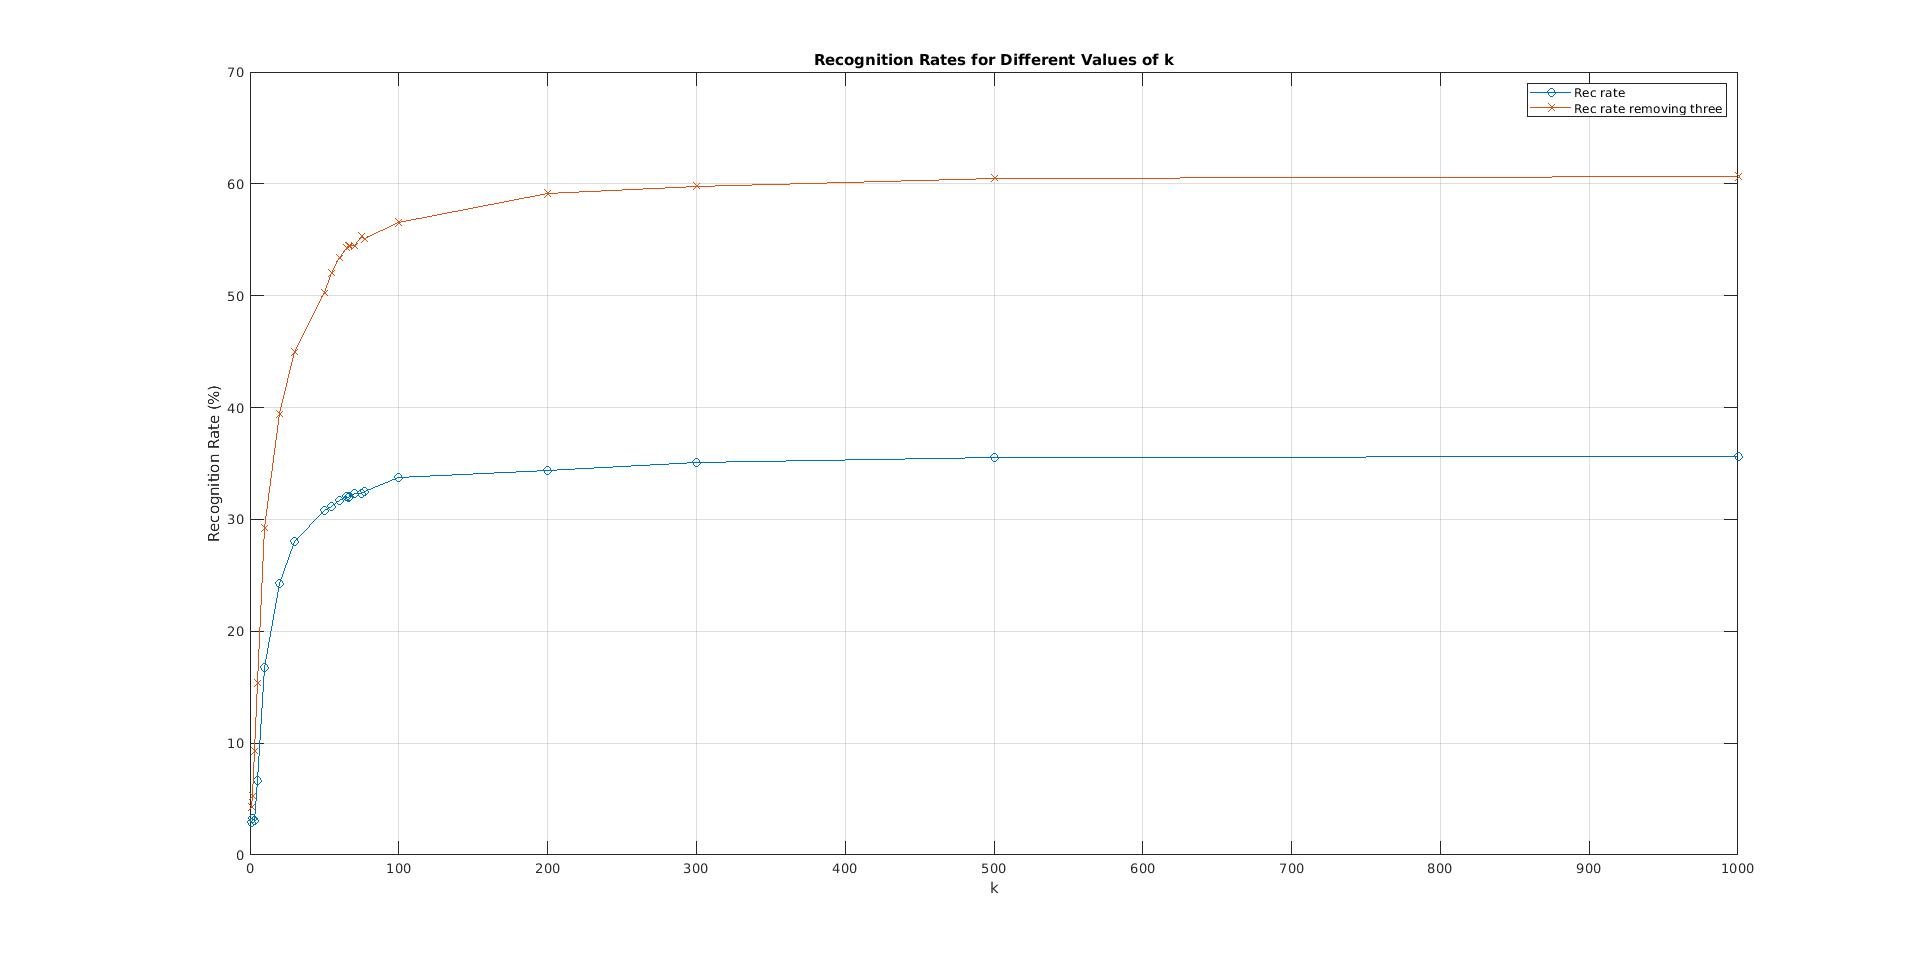
\includegraphics[width=0.8\textwidth]{../images/Yale_dataset_Recognition_Rates_for_diff_k.jpg}
            \caption{Recognition rate vs. k using EIG function for Yale dataset}
        \end{figure}
    \end{itemize}
There's significant improvement in the recognition rate upon removing the eigen coefficients corresponding to top 3 eigen values.
This may be caused by filtering of the data upon removing the top 3 eigen values, thus removing unnecessry artifacts and hence making the model more generalizable. Though it would lead to worse reconstruction accuracy at the cost of improved recognition rate.
\newpage
\subsection{Reconstruction of Face Image:}
Here are the results of implementing reconstruction algorithm for an individual face image in the ORL dataset for $k \epsilon \{2, 10, 20, 50, 75, 100, 125, 150, 175\}$
\begin{figure}[H]
    \centering
    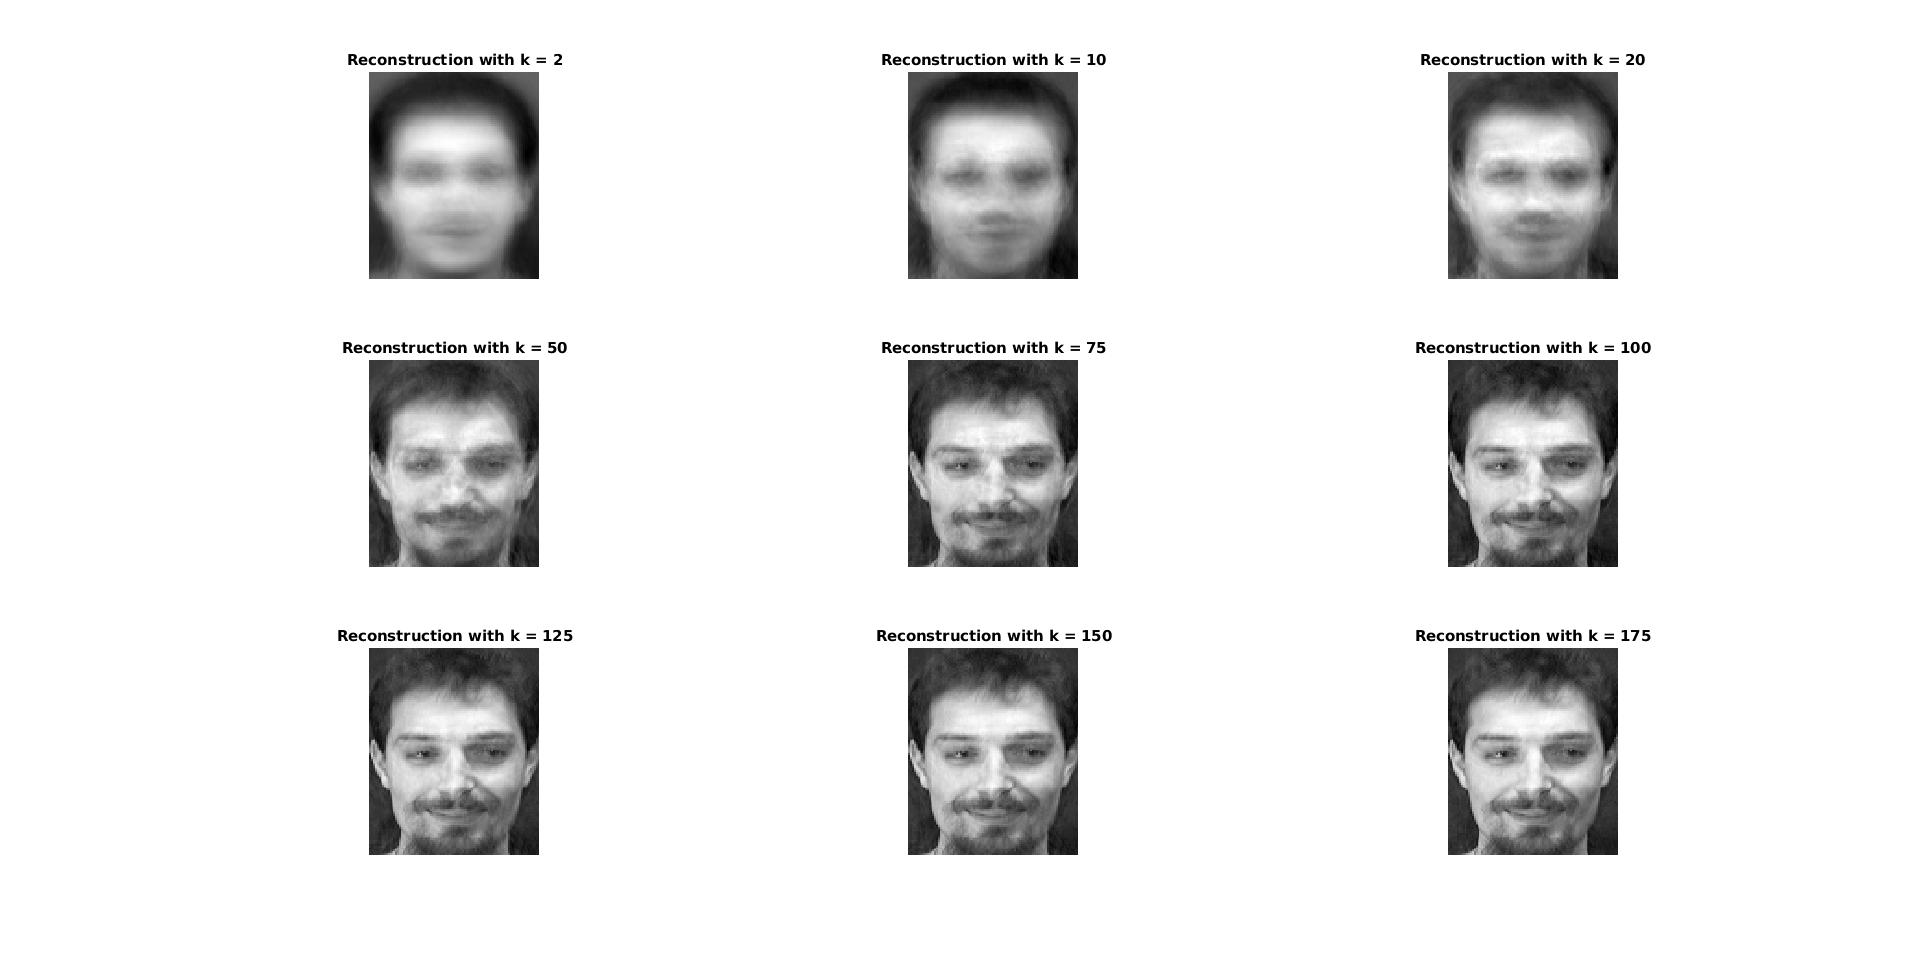
\includegraphics[width=1\linewidth]{../images/Reconstruction_for_different_k.jpg}
    \caption{Reconstruction performance for different k}
    \label{fig:enter-label}
\end{figure}
As expected, increasing k decreases reconstruction loss as we are better able to capture all the features of the face in projected eigen space.\\
\subsection{Eigenfaces corresponding to top-25 (by size) eigen values:}
\begin{figure}[H]
    \centering
    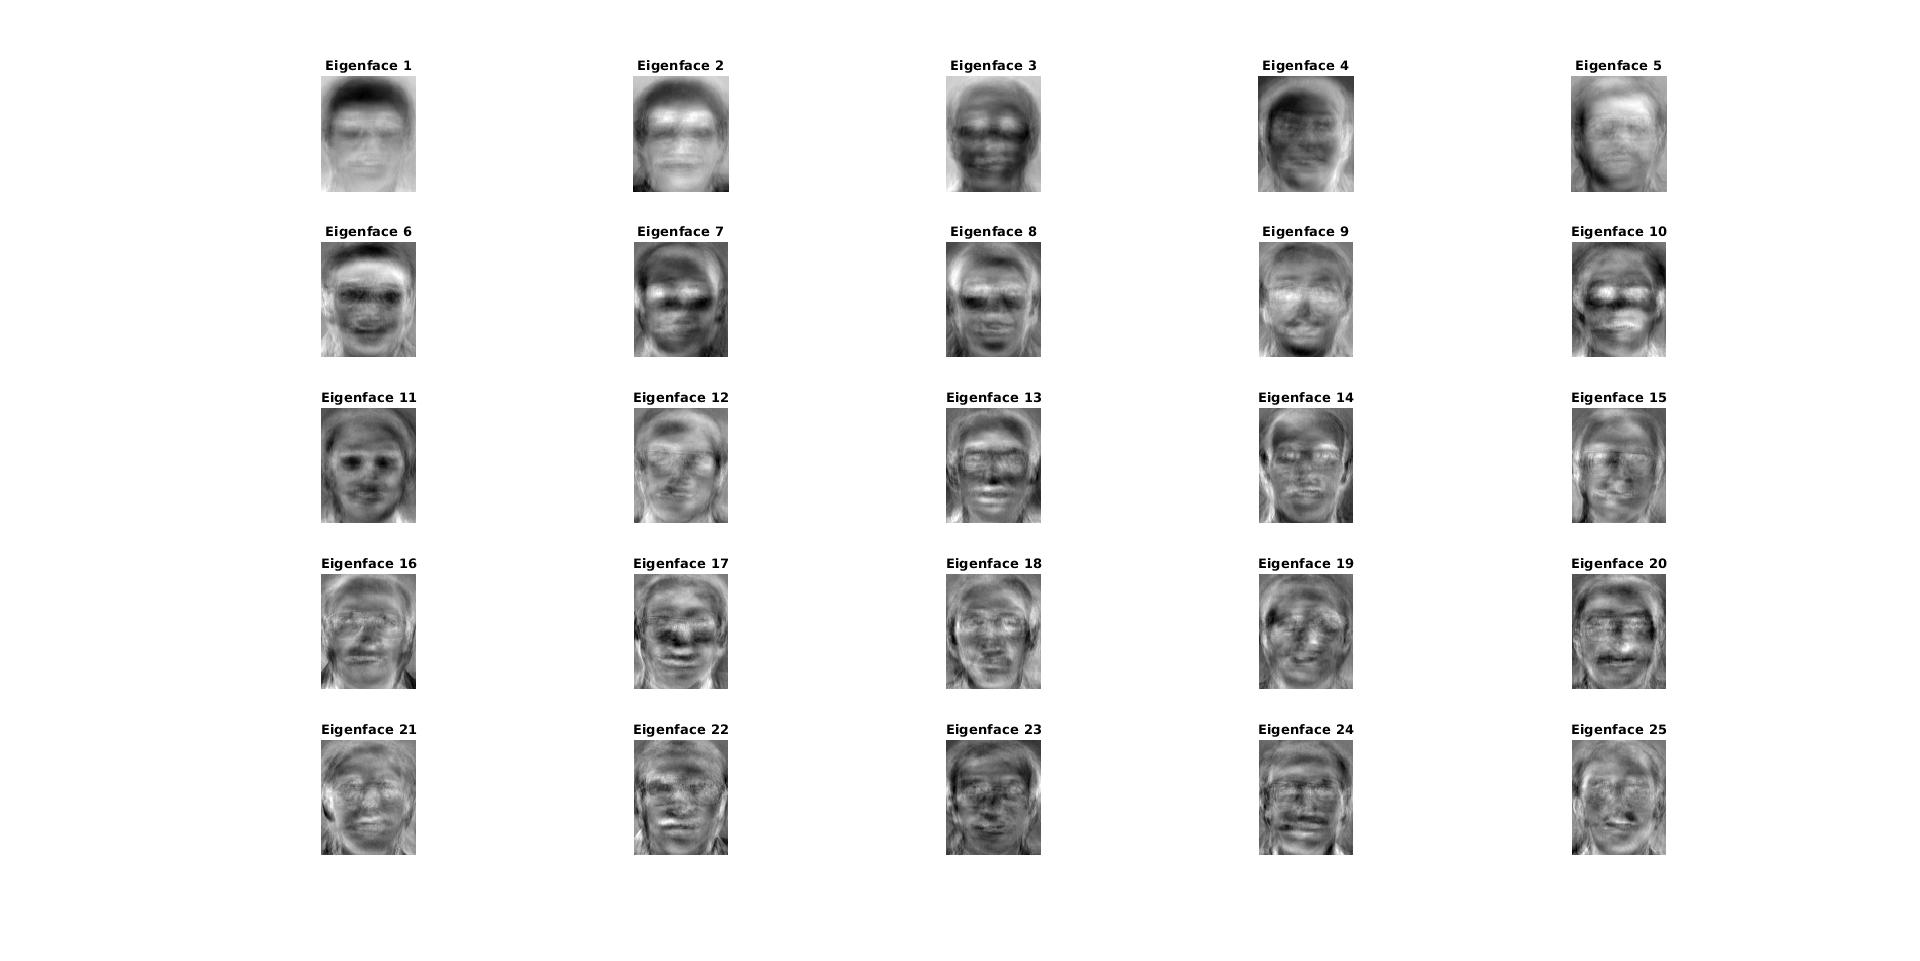
\includegraphics[width = 1.1\linewidth]{../images/Eigenfaces.jpg}
    \caption{Eigenfaces corresponding to the 25 largest eigen values}
    \label{fig:enter-label}
\end{figure}

\end{enumerate}
\end{document}
